% Example template for using the unmeethesis style
% This example is for a Master's candidate in Mathematics
% It contains examples of front matter and most sections that the

% typical graduate student would need to include
% By: N. Doren 02/10/00
%     Minor mods by N. Doren 08/26/11

% Use the following specification for BOTTOM page numbering:
\documentclass[botnum, fleqn, 12]{unmeethesis}
                 % OR
% Use the following specification for TOP page numbering:
% \documentclass[fleqn]{unmeethesis}

\usepackage[utf8]{inputenc}
\usepackage[english]{babel}
\usepackage{amsthm}
\usepackage{amsmath}
\usepackage{amsfonts}
\usepackage{amssymb}
\usepackage{graphicx}
\usepackage{hyperref}
\usepackage{listings}
\usepackage{algpseudocode}
\usepackage{algorithm}

\lstset
{ %Formatting for code in appendix
    language=Matlab,
    basicstyle=\footnotesize,
    numbers=left,
    stepnumber=1,
    showstringspaces=false,
    tabsize=1,    
    breaklines=true,
    breakatwhitespace=false,
}
% Keywords command
\providecommand{\keywords}[1]
{
  \small	
  \textbf{\textit{Keywords---}} #1
}

\newcommand{\real}[0]{\mathbb{R}}
\newcommand{\integer}[0]{\mathbb{Z}}
\newcommand{\nat}[0]{\mathbb{N}}
\newcommand{\grob}[0]{Gr\"obner }
\newcommand{\bigO}[1]{$\mathcal{O}(#1)$}

\newcommand{\separationline}[0]{0.75}

\newtheorem{theorem}{Theorem}[section]
\newtheorem{corollary}{Corollary}[theorem]
\newtheorem{lemma}[theorem]{Lemma}
\newtheorem{definition}{Definition}[section]
\newtheorem{example}{Example}[definition]

\begin{document}

\frontmatter

% Uncomment the next command if you see weird paragraph spacing:
% That is, if you see paragraphs float with lots of white space
% in between them:

% \setlength{\parskip}{0.30cm}

\title{Efficient implementation of interpolation algorithms
for the theories of quantifier-free equality with uninterpreted functions, unit two variable per inequality, and its combination}

\author{Jos\'e Abel Castellanos Joo}

\degreesubject{M.S., Computer Science}

\degree{Master of Science \\ Computer Science}

\documenttype{Thesis}

\previousdegrees{B.Tech., Universidad de las Am\'ericas Puebla, 2015}

\date{July, \thisyear}

\maketitle

%\makecopyright
%Copyright page is no longer necessary D. Murrell

\begin{dedication}
  TODO
\end{dedication}

\begin{acknowledgments}
  \vspace{1.1in}
  TODO
\end{acknowledgments}

%%% Local Variables:
%%% mode: latex
%%% TeX-master: "main"
%%% End:


\maketitleabstract %(required even though there's no abstract title anymore)

\begin{abstract}
  This thesis discusses theoretical aspects and an implementation 
  for the interpolation problem of the following theories: (quantifier-free) equalitiy with uninterpreted
  functions (EUF), unit two variable per inequality (UTVPI), and the combination of the two previous theories. The interpolation algorithms implemented in this thesis are originally proposed in \cite{KAPUR2017}. 

  Refutational proof-based solutions are the usual approach of many interpolation algorithms \cite{10.1007/978-3-642-00768-2_34, mcmillan2011interpolants, 10.1007/978-3-540-24730-2_2}. The approach taken in \cite{KAPUR2017} relies on quantifier-elimination heuristics to construct an interpolant using one of the two formulas involved in the interpolation problem. The latter makes possible to study the complexity of the algorithms obtained. On the other hand, the combination method implemented in this thesis uses a Nelson-Oppen framework, thus we still require for this particular situation a refutational proof in order to guide the construction of the interpolant for the combined theory.

  The implementation uses Z3 \cite{10.1007/978-3-540-78800-3_24} for parsing purposes and satisfiability checking in the combination component of the thesis. Minor modifications were  applied to the Z3's enode data structure in order to label and distinguish formulas efficiently (i.e. distinguish A-part, B-part). Thus, the project can easily be integrated to the Z3 solver to extend its functionality for verification purposes using the Z3 plug-in module.

\clearpage %(required for 1-page abstract)
\end{abstract}


%%% Local Variables:
%%% mode: latex
%%% TeX-master: "main"
%%% End:


\tableofcontents
\listoffigures
\listoftables

\begin{glossary}{Longest  string}
\item TODO.
%\item[$a_{lm}$]
  %Taylor series coefficients, where $l,m = \{0..2\}$
%\item[$A_{\bf{p}}$]
  %Complex-valued scalar denoting the amplitude and phase.
%\item[$A^T$]
  %Transpose of some relativity matrix.
\end{glossary}


%%% Local Variables:
%%% mode: latex
%%% TeX-master: "main"
%%% End:


\mainmatter

\chapter{Introduction}

Modern society is witness of the impact computer software 
has done in recent years. The benefits of this massive 
automation is endless. On the other hand, when software 
fails, it becomes a catostrophe ranging from economic loss
to threats for human life. 

Due to strict and ambitious agendas, many software products
are shipped with unseen and unintentional bugs which might potentially put
at risk people's life like critical systems. Several approaches have been 
used to improve software quality. However, many of these approaches 
offer partial coverage or might take an abyssal amount of human effort to 
provide such solutions. Thus, these approaches cannot be consideral practical. 
On the other hand, for certain applications these contributions are relevant
and their proper use fit such workflows uniquely.

Formal methods aim to bring a unique combination of automation, rigor, and 
efficiency (whenever effecient algorithms exits for the verification task
). This thesis discusses a particular problem in software verification
known as \emph{the interpolantion problem} for the theories of the quantifier-free
fragment of equality with uninterpreted functions (EUF) and unit two variable per
inequality (UTVPI) and their combination. These two theories have been 
studied extensively and researcher have found several applications for them. 

\section{Backgroud}

An interpolant of a pair of logical formulas $(\alpha, \beta)$ 
is a logical formula $\gamma$
such that $\alpha$ implies $\gamma$, $\beta \land \gamma$ is logically
inconsistent, and $\gamma$ only has common symbols of $\alpha$ and $\beta$.
Informally this means that the 
interpolant `belongs' to the consequence of $\alpha$, 
and `avoids' being part of the consequence of $\beta$. 
Not surprisingly, this intuition is behind many software verification 
routines where the first formula models a desirable state/property
(termination, correctness) of a computer program, and the second 
formula models the set of undesirable states (non-termination, 
errors, crashes, etc) of such software. In Chapter 
\ref{preliminaries}, an extensive review of the formal concept 
is provided.

Eventhough interpolants are not a direct concern in verification
problems, these problems are found in the core algorithms of the 
following two applications:

\begin{itemize}
  \item Refinement of abstract models: In order to improve 
    coverage and decrease the complexity in verification problems,
    abstract interpretation has become a proper technique to 
    accomplish the latter together with model checking. Eventhough the
    methodology provides sound results, it is certainly not complete.
    Additionally, several abstractions do not capture the semantical
    meaning of programs due to the \emph{over-approximation} approach.
    Hence, interpolants are used to strength predicate
    abstractions by using interpolants constructed from valid 
    traces in the abstract model but not valid in the actual model
    (\emph{spurious counterexamples}) \cite{10.1145/876638.876643,
    10.1007/978-3-540-45069-6_1, 10.1145/982962.964021}.
  \item Invariant generation: following the same idea as in the previous
    case, \emph{if a fix point is obtained in the refinement process},
    we can obtain a logical invariant of computer programs 
    \footnote{The interpolation
      generation approach discussed can be understood as a \emph{lazy framework}
      similarly to SAT/SMT algorithms. The former is
      about the production of interpolants, the latter is for 
      assignments/models respectively. Both \emph{block/learn} the formulas
    in order to find their results.}
    Situations where this happens might be due to the finiteness of possible 
    states in the program. It is worth mentioning that the 
    invariant problem as stated in \cite{10.1145/363235.363259} 
    is undecidable \cite{10.2307/1990888, 10.1145/371282.371285}.
\end{itemize}

\section{Related work}

There are several interpolation algorithms for the theories
involved in the thesis work. The approaches can be classified
into the following categories:

\begin{itemize}
  \item Proof-based approach: This category relies on the availability
    of a refutational proof.  The interpolant is constructed using a
    recursive function over the structure of the proof
    tree. In \cite{10.1007/978-3-540-24730-2_2,mcmillan2011interpolants}
    the author defines an interpolation calculus. This particular
    approach uses a proof tree produced by the SMT solver Z3 
    and does not need to modify any of Z3's internal mechanisms.
    Among the advantages of this approach is that
    theory combination is given for free since the SMT solver takes care of this
    problem. On the other hand, Z3's
    satellities theories are not sufficiently integrated with its
    proof-producing mechanism. Hence, one can find $\mathcal{T}-lemmas$
    as black-boxes which introduces incompleteness in the
    interpolation calculus. For completeness, these lemmas are 
    solved separately by another interpolantion algorithm for the respective
    theory. 
    In \cite{10.1007/11532231_26} the authors provide a Nelson-Oppen framework
    to compute interpolants. For the convex-case, the approach only 
    exchange equalities as required by the Nelson-Oppen framework. For
    the non-convex case, the authors require a resolution-based refutational proof
    to compute interpolants using Pudlak's algorithm. The introduction of the
    class of \emph{equality interpolanting theories} is 
    considered among the most relevant contributions of the paper 
    by the verification community. This is property about theories which states
    that if a theory is capable of proving a mixed equality $a = b$ (an equality
    which contains symbols from the two formulas in the interpolanting problem)
    then it exists a common term in the language of the theory $t$ (known as
    the interpolating-term) such that 
    the theory can prove $a = t$ and $t = b$. The property facilities 
    formula-splitting for interpolation purposes.
    In \cite{10.1007/978-3-642-00768-2_34} the authors modify a 
    resolution-based refutational proof by introducing common-terms in 
    the proof in order to produce interpolants in what is called
    colorable-proofs, which are proof trees which do not contained AB-mixed
    literals. This is pointed as an improvement to the approach followed 
    in \cite{10.1007/11532231_26} which executes a similar idea but done 
    progressively as the proof-tree is built and does not require 
    the theories solver to be \emph{equality propagating} 
    \footnote{The authors in \cite{10.1007/11532231_26} require that 
      the theory solvers keep track of the interpolating-term 
      and propagate this term whenever
    possible}. 
    However, this results is not generalizable
    to non-convex theories due to internal constraints.

  \item Reduction-based approach: This method transforms the interpolation
    problem into a query for some solver related to the theory. 
    An example of this approach can be found in \cite{10.1007/978-3-540-69738-1_25}
    where the authors use a linear-inequality solver to provide an interpolant
    fot the theory of linear inequalities over the rational/real numbers 
    ($LIA(\mathbb{Q})/LIA(\mathbb{R})$). 
    Additionally, they integrate the procedure with a 
    \emph{hierarchial reasoning} approach in order to incorporate 
    the signature of theory for (quantifer-free) equalities with uninterpreted 
    functions.
\end{itemize}

\section{Outline of the thesis}

\begin{itemize}
  \item Chapter 2 provides an extensive background 
    of fundamentals ideas, definitions and decision procedures 
    used in the thesis work.
  \item Chapters 3, 4, and 5 explain implentation details
    of the interpolating algorithms for the theories
    EUF, UTVPI, and their combination respectively. These
    chapters share the same structure. They start with the
    algorithms used to solve the interpolation problem, discuss
    about implementation details including diagrams
    of the architecture of the implemented system, and 
    show a performance comparision with the iZ3 interpolation 
    tool available in the SMT solver Z3 until version 4.7.0.
\end{itemize} 

\section{Contributions}

The contributions of the thesis can be summarized as follow:

\begin{itemize}
  \item[1.] Implementation of the interpolation algorithm for the theory EUF 
    proposed in \cite{KAPUR2017}.
  \item[2.] Formulation and implementation of a new 
    procedure for checking unsatisfiability of grounded equations in 
    Horn clauses using a congruence closure algorithm with explanations
    used in the implementation of item 1.
  \item[3.] Implementation of the interpolation algorithm for the theory UTVPI
    proposed in \cite{KAPUR2017}.
  \item[4.] Implementation of the combination procedure for interpolating
    algorithm proposed in \cite{10.1007/11532231_26} in order to 
    combine the implementations of items 1. and item 3.
\end{itemize}

%%% Local Variables:
%%% mode: latex
%%% TeX-master: "main"
%%% End:

\chapter {Preliminaries} \label{preliminaries}

This chapter discusses basic concepts from first-order logic that are used in the rest of this thesis. We will pay particular attention to their language and semantics since these are fundamental concepts necessary to understand the algorithmic constructions to compute interpolants. For a comprehensive treatment on the topic, the reader is suggested the following references \cite{10.5555/1642730, DBLP:books/daglib/0076838}.

\section{First-Order Predicate Logic}

\subsection{Language}
A language is a collection of symbols of different sorts equipped with a rule of composition that effectively tells us how to recognize elements that belong to the language \cite{DBLP:books/daglib/0080654}. In particular, a first-order language is a language that expresses boolean combinations of predicates using terms (constant symbols and function applications). In mathematical terms, 

\begin{definition}
 A first-order language (also denoted signature) is a triple $\langle \mathfrak{C}, \mathfrak{P}, \mathfrak{F} \rangle$ of non-logical symbols where:

\begin{itemize}
  \item $\mathfrak{C}$ is a collection of constant symbols
  \item $\mathfrak{P}$ is a collection of n-place predicate symbols
  \item $\mathfrak{F}$ is a collection of n-place function symbols
\end{itemize}

including logical symbols like quantifiers(universal ($\forall$), existential($\exists$)) logical symbols like parenthesis, propositional connectives (implication ($\rightarrow$), conjunction ($\land$), disjunction ($\lor$), negation ($\neg$)), and a countable number of variables \emph{Vars} (i.e. $\emph{Vars} = \{v_1, v_2, \dots\}$).

The rules of composition distinguish two objects, \emph{terms} and \emph{formulas}, which are defined recursively as follows:

\begin{itemize}
  \item Any variable symbol or constant symbol is a term.
  \item If $t_1, \dots, t_n$ are terms and $f$ is an n-ary function symbol, then $f(t_1, \dots, t_n)$ is also a term.
  \item If $t_1, \dots, t_n$ are terms and $P$ is an n-ary predicate symbol, then $P(t_1, \dots, t_n)$ is formula.
  \item If $x$ is a variable and $\psi, \varphi$ are formulas, 
    then $(\neg \psi), (\forall x . \psi), (\exists x . \psi)$ 
    and $(\psi \square \varphi)$ are formulas where $\square \in \{\rightarrow, \land, \lor\}$
  \item No other expression in the language can be considered terms nor formulas if such expressions are not obtained by the previous rules.
\end{itemize}

For notation purposes, we compactly represent a tuple $\langle x_1, \dots, x_n \rangle$ of variables as
$\cev{x}$. Abusing the notation, a formula of the form 
$\forall \cev{x} . \phi(\cev{x})$ (resp. $\exists \cev{x} . \phi(\cev{x})$)
denotes the formula $\forall x_1 . \forall x_2 \dots \forall x_n . \phi(x_1, \dots, x_n)$
(resp. $\exists x_1 . \exists x_2 \dots \exists x_n . \phi(x_1, \dots, x_n)$)

\end{definition}

\subsection{Semantics}

In order to define a notion of truth in a first-order language, it is necessary to 
associate for each non-logical symbol (since logical symbols have established 
semantics from propositional logic) a denotation or mathematical object and 
an \emph{assignment} to the collection of variables. The two previous 
components are part of a \emph{structure} \cite{DBLP:books/daglib/0076838} 
(or interpretation \cite{DBLP:books/daglib/0080654}) for a first-order language.

\begin{definition}
  Given a first-order language $\mathfrak{L}$, an interpretation $\mathfrak{I}$ is a pair $(\mathfrak{A}, \mathfrak{J})$, where $\mathfrak{A}$ is a non-empty domain (set of elements) and $\mathfrak{J}$ is a map that associates to the non-logical symbols from $\mathfrak{L}$ the following elements:
  \begin{itemize}
    \item $\mathfrak{I}$ assigns to each constant symbol $c$
      an elements $c^\mathfrak{A} \in \mathfrak{A}$
    \item $\mathfrak{I}$ assigns to each n-place
      predicate symbol $P$ an n-ary relation 
      $P^{\mathfrak{A}} \subseteq \mathfrak{A}^n$
    \item $\mathfrak{I}$ assigns to each n-place function
      symbol $f$ an n-ary operation $f^\mathfrak{A}$
      on $\mathfrak{A}$, i.e. $f^\mathfrak{A} : 
      \mathfrak{A}^n \rightarrow \mathfrak{A}$
  \end{itemize}

  An assignment $s : Vars \rightarrow \mathfrak{A}$ is a 
  map between variables to elements from the domain of 
  the interpretation.
\end{definition}

With the definition of interpretation $\mathfrak{I}$ and assignment $s$, we can recursively define a notion of \emph{satisfiability} (denoted by the symbol $\models_{\mathfrak{I}, s} $) as a free extension from atomic predicates (function application of predicates) to general formulas as described in \cite{DBLP:books/daglib/0076838}. For the latter, we need to extend the assignment function to all terms in the language.

\begin{definition}
  Let $\mathfrak{I} = (\mathfrak{A}, \mathfrak{J})$ be an interpretation and $s$ an assignment for a given language,
  Let $\bar{s} : Terms \rightarrow A$ be defined recursively as follows:
  \begin{itemize}
    \item $\bar{s}(c) = c^\mathfrak{J}$
    \item $\bar{s}(f(t_1, \dots, t_n)) = f^\mathfrak{J}(\bar{s}(t_1), \dots, \bar{s}(t_n))$
  \end{itemize}
\end{definition}

Notice that the extension of $s$ depends on the interpretation used.

\begin{definition}
  Given an interpretation $\mathfrak{I} = (\mathfrak{A}, \mathfrak{J})$, an assignment $s$, and $\psi$ a formula, we define $\mathfrak{I} \models_s \psi$ (read $\psi$ is satisfiable under interpretation $\mathfrak{I}$ and assignment $s$) recursively as follows:
  \begin{itemize}
    \item $\models_{\mathfrak{I}, s} P(t_1, \dots, t_n)$ 
      if and only if 
      $\langle
      \bar{s}(t_1), \dots, \bar{s}(t_n) \rangle 
      \in P^{\mathfrak{J}}$
    \item $\models_{\mathfrak{I}, s} \neg \psi$ if and only if  it is not the case that $\models_{\mathfrak{I}, s}   \psi$
    \item $\models_{\mathfrak{I}, s} \psi \land \varphi$ if and only if $\models_{\mathfrak{I}, s}  \psi$ and $   \models_{\mathfrak{I}, s}  \varphi$
    \item $   \models_{\mathfrak{I}, s}  \psi \lor \varphi$ if and only if $   \models_{\mathfrak{I}, s}  \psi$ or $   \models_{\mathfrak{I}, s}  \varphi$
    \item $   \models_{\mathfrak{I}, s}  \psi \rightarrow \varphi$ if and only if $   \models_{\mathfrak{I}, s}  \neg \psi$ or $   \models_{\mathfrak{I}, s}  \varphi$
    \item $   \models_{\mathfrak{I}, s}  \forall x . \psi$ if and only if for every $d \in \mathfrak{A},    \models_{\mathfrak{I}, s_{x \mapsto d}} \psi$, where $s_{x \mapsto d} : Vars \rightarrow \mathfrak{A}$ is reduct of $s$ under $Vars \setminus \{x\}$ and $s_{x \mapsto d}(x) = d$
    \item $   \models_{\mathfrak{I}, s}  \exists x . \psi$ if and only if exits $d \in \mathfrak{A},    \models_{\mathfrak{I}, s_{x \mapsto d}} \psi$, where $s_{x \mapsto d}$ is defined as in the previous item.
  \end{itemize}

  If an interpretation and assignment satisfies a formula, then we 
  say that the interpretation and the assignment are a model for the 
  respective formula. A collection of formulas is satisfied by 
  an interpretation and assignment if these model each formula 
  in the collection.

  A formula $\psi$ is said to be a \emph{valid} 
  formula of the interpretation $\mathfrak{I}$ 
  when $\models_{\mathfrak{I}, s} \psi$ for all 
  possible assignments $s$.

  Additionally, if all the models $(\mathfrak{I},
  s)$ in a language of a collection of formulas 
  $\Gamma$ satisfy a formula $\psi$, then we say 
  that $\Gamma$ logically implies $\psi$ 
  (written $\Gamma \models \psi$). For the 
  latter, $\psi$ is said to be a \emph{valid} 
  formula of the model $(\mathfrak{I}, s)$.

\end{definition}

%%% Local Variables:
%%% mode: latex
%%% TeX-master: "main"
%%% End:

\section{Mathematical Theories} \label{math_theories}

A theory $\mathcal{T}$ is a collection of formulas that are closed under logical implication, i.e. if $\mathcal{T} \models \psi$ then $\psi \in \mathcal{T}$. This concept is quite relevant for our thesis work since we will focus on two theories, the quantifier-free fragment of the theory of equality with uninterpreted functions (EUF), and the theory of unit two variable per inequality (UTVPI). 

For some theories it is enough to provide a collection of formulas (known as the axioms of the theory). For the case of the theories of interest for the thesis, the axiomatization if the following:

\subsection{Equality with uninterpreted functions}

\begin{definition} \label{euf_axioms}
  Let $\mathfrak{L}_{EUF} = \{ \{\}, \{ = \}, \{ f_1, \dots, f_n \} \}$ be the language of EUF. The axioms of the theory are:
  \begin{itemize}
    \item (Reflexivity) $\forall x . x = x$
    \item (Symmetry) $\forall x . \forall y . x = y \rightarrow y = x$
    \item (Transitivity) $\forall x . \forall y . \forall z. (x = y \land y = z) \rightarrow x = z$
    \item (Congruence) $\forall x_1  \dots \forall x_n . \forall y_1 \dots \forall y_n . (x_1 = y_1 \land \dots \land x_n = y_n) \rightarrow f(x_1, \dots, x_n) = f(y_1, \dots, y_n) $
  \end{itemize}
\end{definition}

We notice that the congruence axiom is not a first-order logic axiom, but rather an axiom-scheme since it is necessary to \emph{instantiate} such axiom for every arity of the function symbols in a given language.

\subsection{Ordered commutative rings}

In order to describe the UTVPI theory we will first introduce the language and theory of an ordered commutative ring.

\begin{definition}
  Let $\mathfrak{L}_{Ord-R} = \{, \{0, 1 \}, \{ = , \leq \}, \{+, -, * \}, \}$ be the 
  language of an ordered commutative ring $R$. The axioms of the theory are:
  \begin{itemize}
    \item $\forall x . \forall y . \forall z . x + (y + z) = (x + y) + z$
    \item $\forall x . \forall y .  x + y = y + x$
    \item $\forall x . x + 0 = x$
    \item $\forall x . x + (- x) = 0$
    \item $\forall x . \forall y . \forall z. x * (y * z) = (x * y) * z$
    \item $\forall x . x * 1 = x$
    \item $\forall x . \forall y .  x * y = y * x$
    \item $\forall x . \forall y . \forall z . x * (y + z) = x * y + x * z$
    \item $\forall x . \forall y . \forall z . (y + z) * x = y*x + z * x$
    \item $\forall x . \forall y . \forall z . x \leq y \rightarrow x + z \leq y + z$
    \item $\forall x . \forall y . (0 \leq x \land 0 \leq y) \rightarrow 0 \leq x * y$.
    \item $0 \neq 1 \land 0 \leq 1$ 
  \end{itemize}
\end{definition}

Section \ref{decision_procedures} discusses computability 
aspects for the theories of interest that are relevant 
for verification.

%%% Local Variables:
%%% mode: latex
%%% TeX-master: "main"
%%% End:

\section{Interpolants}

Following the notation in \cite{10.1007/11532231_26}, we denote 
$\mathcal{V}(\psi)$ to be the set of non-logical symbols, variables
and constants of formula $\psi$. Given an instance for the interpolation
problem $(A, B)$ \footnote{For the rest of the thesis, we will denote the 
  first formula of an interpolation problem as the A-part 
and the second component as the B-part}, 
we distinguish the following categories:

\begin{itemize}
  \item $\psi$ is \emph{A-local} if $\mathcal{V}(\psi) \in 
    \mathcal{V}(A) \setminus \mathcal{V}(B)$
  \item $\psi$ is \emph{B-local} if $\mathcal{V}(\psi) \in 
    \mathcal{V}(B) \setminus \mathcal{V}(A)$
  \item $\psi$ is \emph{AB-common} if $\mathcal{V}(\psi) \in
    \mathcal{V}(A) \cap \mathcal{V}(B)$
  \item $\psi$ is \emph{AB-pure} when either $\mathcal{V}(\psi) \subseteq 
    \mathcal{V}(A)$ or $\mathcal{V}(\psi) \subseteq \mathcal{V}(B)$, otherwise
    $\psi$ is \emph{AB-mixed}
\end{itemize}

\begin{example} \label{first_example}

  Consider the following interpolation pair: $(f(a + 2) + 1 = c + 1
    \land f(a + 2) = 0
  , f(c) \leq b \land b < f(0))$. With respect to the previous 
  interpolation pair, we can tell that:
  \begin{itemize}
    \item The formula $f(a + 2) = c$ is 
      AB-pure but not A-local nor B-local nor AB-common
    \item The formula $\neg(a \leq f(f(b) + 1))$ is an AB-mixed
      literal
    \item The formula $a + 1 = 1$ is A-local.
    \item The formula $c + 1 = 1$ is AB-pure but not AB-common.
    \item The formula $c = 0$ is AB-common.
    \item In general, $AB-common$ formulas are not $AB-pure$ formulas.
  \end{itemize}
\end{example}

\subsection{Craig interpolation theorem}

Let $\alpha, \beta, \gamma$ be logical formulas in a given theory. If
$\models_{\mathcal{T}} \alpha \rightarrow \beta$, we say that $\gamma$ is an
interpolant for the interpolation pair $(\alpha, \beta)$ if the following conditions
are met:

\begin{itemize}
\item $\models_{\mathcal{T}} \alpha \rightarrow \gamma$
\item $\models_{\mathcal{T}} \gamma \rightarrow \beta$
\item Every non-logical symbol in $\gamma$ occurs both in $\alpha$ and
  $\beta$.
\end{itemize}

The \emph{interpolation problem} can be stated naturally as 
follows: given two logical formulas $\alpha, \beta$ such that 
$\models_{\mathcal{T}} \alpha \rightarrow \beta$, find
the interpolant for the pair $(\alpha, \beta)$.

In his celebrated result \cite{10.2307/2963594}, Craig proved that for every pair
$(\alpha, \beta)$ of formulas in first-order logic such that
$\models \alpha \rightarrow \beta$, an interpolation formula exists. Nonetheless,
there are many logics and theories that this result does not hold \cite{komori1978}.

Usually, we see the interpolation problem defined differently in the literature, 
where it is considered $\beta^{'}$ to be $\neg \beta$ and 
the problem requires that the pair $(\alpha, \beta^{'})$
is mutually contradictory (unsatisfiable). This definition was popularized by 
McMillan \cite{10.1007/978-3-540-24730-2_2}. This shift of attention explains 
partially the further development in interpolation generation algorithms 
since many of these relied on SMT solvers that provided refutation proofs 
in order to (re)construct interpolants for different theories (and their 
combination) \cite{10.1007/978-3-642-02959-2_17, 
10.1007/978-3-642-36742-7_9, mcmillan2011interpolants}.

Relaxed definitions are considered to the interpolation 
problem when dealing with specific
theories \cite{10.1007/11532231_26} in a way that interpreted 
function can be also part of the interpolant. The latter is 
justified since otherwise, many interpolation formulas might not exist
in different theories or the interpolants obtained might not 
be relevant (for example, lisp programs). This is formalized as follows:

\begin{definition} \cite{10.1007/11532231_26}
  Let $\mathcal{T}$ be a first-order theory of a signature $\Sigma$ and 
  let $\mathcal{L}$ be the class of quantifier-free $\Sigma$ formulas.
  Let $\Sigma_\mathcal{T} \subseteq \Sigma$ denote a designated set
  of interpreted symbols in $\mathcal{T}$. Let $A, B$ be formulas
  in $\mathcal{L}$ such that $A \land B \models_{\mathcal{T}} \bot$.
  A \emph{theory-specific} interpolant for $(A, B)$ in $\mathcal{T}$
  is a formula $I$ in $\mathcal{L}$ such that 
  $A \models_{\mathcal{T}} I$, $B \land I \models_{\mathcal{T}} \bot$,
  and $I$ refers only to AB-common symbols and symbols in 
  $\Sigma_{\mathcal{T}}$.
\end{definition}

\begin{example}
  In example \ref{first_example} we can tell $c + 1 = 1$ is not an
  interpolant simplify because the symbol $1$ only appears on the
  A-part. However, if $\Sigma_{\mathcal{LIA(\mathbb{Z})}}$ contains the
  interpreted symbols of $LIA(\mathbb{Z})$ (i.e. $+, *, 0, 1, 2, \dots$),
  then $c + 1 = 1$ becomes a \emph{theory-specific} interpolant. 

  Notice that $c = 0$ is an interpolant even if the set of interpreted symbols 
  used for interpolation is empty.
\end{example}

\subsection{Uniform Interpolant}

A uniform interpolant is a particular kind of interpolant for an inconsistent
pair of formulas. Introduced in \cite{pitts1992} as a 
construction to provide an interpretation
for second order intuitionistic propositional logic 
\emph{$IpC^2$}
\footnote{I.e. $IpC^2$ quantifies over 
propositional variables.}
using intuitionistic propositional logic \emph{IpC}.
Our notion of uniform interpolant is taken 
from \cite{ghilardi2020compactly}
where the authors provide the following definition:

\begin{definition}
  Fix a theory $T$ and an existential formula $\exists \cev{e} . \phi(\cev{e}, \cev{z})$; call \emph{residue} of $\exists \cev{e} . \phi(\cev{e}, \cev{z})$ the following set of
  quantifier-free formulae:

  \begin{equation*}
    Res(\exists \cev{e} . \phi(\cev{e}, \cev{z})) = \{ \theta(\cev{z}, \cev{y}) | T \models \exists \cev{e} . \phi(\cev{e}, \cev{z}) \rightarrow \theta(\cev{z}, \cev{y}) \} =\{ \theta(\cev{z}, \cev{y}) | T \models \phi(\cev{e}, \cev{z}) \rightarrow \theta(\cev{z}, \cev{y}) \}
  \end{equation*}

  A quantifier-free formula $\psi(\cev{y})$ is said to be a \emph{T-uniform interpolant} 
  of $\exists \cev{e} . \phi(\cev{e}, \cev{z})$ if and only if $\psi(\cev{y}) \in Res(\exists \cev{e} \phi(\cev{e}, \cev{y}))$ and 
  $\psi(\cev{z})$ implies (modulo T)
  all the other formulae in $Res(\exists \cev{e} \phi(\cev{e}, \cev{y}))$.

  A theory $T$ has the \emph{Uniform Interpolation Property} 
  if every existential formula
  $\exists \cev{e} . \phi(\cev{e},\cev{y})$ has a T-uniform interpolant. 

\end{definition}

%%% Local Variables:
%%% mode: latex
%%% TeX-master: "main"
%%% End:

\section{Decision Procedures} \label{decision_procedures}

Given a theory $\mathcal{T}$ and a formula $\psi$ in 
the language of $\mathcal{T}$, is it possible to know 
$\models_{\mathcal{T}} \psi$? The last question is 
known as the decision problem for 
$\mathcal{T}$. This question has 
been studied extensively for many theories of interest 
\cite{borger2001classical}. 

Regarding the decidability of the theories 
discussed in the thesis work, it is known that 
the quantified EUF theory is undecidable \cite{borger2001classical}
Nonetheless, the quantifier-free fragment of EUF and 
the restriction imposed in the decision problem for 
the UTVPI theory allow efficient algorithms to decide 
validity and satisfiability in their respective theories 
\cite{10.1145/322186.322198, 10.1145/322217.322228, 
10.1007/11559306_9}. The ordered abelian group theory
is decidable as well \cite{DBLP:books/daglib/0076838}.

In the rest of this section we review some decision 
problems and provide references to their respective
decision procedures used in the implementation work of 
the thesis.

\subsection{Satisfiability and Satisfiability Modulo Theories}

The satisfiability problem consists of finding a 
propositional assignment for a propositional formula. 
This problem is at the core level of complexity theory, 
defining an important class of problems known as 
NP, which includes problems whose
algorithms seem to be intractable.
Developments in algorithms and heuristics 
\cite{10.5555/2898950, 
935565} have made it possible to use satisfiability 
algorithms 
to solve real-world problems in 
verification \footnote{These
  advances do not provide an answer to the well-known P vs. NP
  problem. There are results indicating a class of problem instances
  for many of the SAT algorithms which cannot be solved in less that
  \bigO{2^n} steps \cite{10.5555/2898950}.
}.

The DPLL algorithm \cite{10.1145/368273.368557} 
(and other extensions) is the algorithm
found in many SAT solvers. Fundamentally, it is a search-based algorithm
which implements operators (decide, unit-propagation, backtrack)
to find a satisfiable assignment. If the algorithm is not able to
find a satisfying assignment for a formula, then it is possible to 
extract a \emph{resolution proof} based on the traces of the search
operations.

\begin{example}

  \begin{figure}

    \centering

    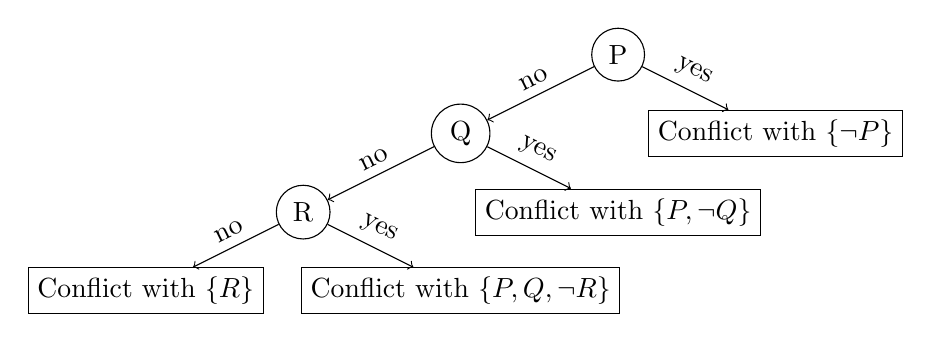
\begin{tikzpicture}[->]
      \node(p) at (6, 5) [circle, draw] {P};
      \node(q) at (4,4) [circle, draw] {Q};
      \node(r) at (2, 3) [circle, draw] {R};
      \node(expl1) at (8, 4) [rectangle, draw] {Conflict with $\{\neg P\}$};
      \node(expl2) at (6, 3) [rectangle, draw] {Conflict with $\{P, \neg Q\}$};
      \node(expl3) at (4, 2) [rectangle, draw] {Conflict with $\{P, Q, \neg R\}$};
      \node(expl4) at (0, 2) [rectangle, draw] {Conflict with $\{R\}$};

      \path[every node/.style={sloped,anchor=south,auto=false}]
      (p) edge node {yes} (expl1)   
      (p) edge node {no}  (q)   
      (q) edge node {yes} (expl2)
      (q) edge node {no}  (r)
      (r) edge node {yes} (expl3)
      (r) edge node {no}  (expl4);
    \end{tikzpicture}

    \caption{Example of DPLL execution on 
      $\{\{\neg P\}, \{P, Q, \neg R\}, \{R\}, 
    \{P, \neg Q\} \}$} \label{dpll_figure}

  \end{figure}

  We can see that the following resolution proof resembles the
  structure of the DPLL execution on figure \ref{dpll_figure}, i.e.
  if we rotate the proof-tree and mark the nodes by the pivots used
  we obtained a similar tree obtained by the execution of the DPLL
  algorithm. This fact becomes relevant because it enables us 
  to construct a resolution proof from the traces of a SAT 
  solver used
  in the theory combination part of the implementation. 

  \begin{figure}
    \centering
    \begin{prooftree}
      \hypo[]{\neg P}
      \hypo[]{P \lor Q \lor \neg R}
      \infer2[$res_P$]{Q \lor \neg R}
      \hypo[]{R}
      \infer2[$res_R$]{Q}
      \hypo[]{P \lor \neg Q}
      \infer2[$res_Q$]{P}
      \hypo[]{\neg P}
      \infer2[$res_P$]{\bot}
    \end{prooftree}
    \caption{Example of resolution proof} 
    \label{example_resolution_proof}
  \end{figure}

\end{example}

We can extend this approach to work not only with propositional
variables but with terms of more complex signatures 
\cite{10.5555/1391237}. If we are given a boolean combination 
of formulas from any theory that is capable of deciding the 
satisfiability of any conjunction of formulas in the theory, 
by using a \emph{lazy framework} integration with a SAT solver it is 
possible to find either a model or declare unsatisfiable such boolean
combination as follows: (i) first abstract the literals in the boolean
combination to (pseudo) boolean propositions; (ii) find a satisfying
assignment (using a SAT solver) of the (pseudo) boolean propositions;
(iii) using the theory solver, test if the collection of positive
and negative literals induced by the pseudo boolean variables is
satisfiable; (iv) if it is then declare the formula satisfiable, 
otherwise \emph{learn} (or block) the pseudo boolean clause obtained
(by negating the conjunction of boolean constraints) in the SAT
solver and repeat from step (ii); (v) if it is not possible to
find a satisfying assignment for the pseudo boolean variables, 
declare the original formula to be unsatisfiable.

These algorithms are used in the last section of the thesis work.
The implementation for the interpolation combination method
in \cite{10.1007/11532231_26} requires a resolution-based
proof in order to compute partial interpolants by integrating
Pudlak's algorithm.

%%% Local Variables:
%%% mode: latex
%%% TeX-master: "main"
%%% End:

\subsection{Congruence Closure}

The congruence closure problem consists of given a conjunction of
equalities and disequalities $\psi$ determine if an equality
$u = v$ follows from the consequence generated by $\models_{EUF} 
\psi$.

In \cite{10.1007/978-3-540-32033-3_33}, the authors 
introduced a Union-Find data structure that supports the 
Explanation operation. This operation receives as input 
an equation between constants. If the input equation is 
a consequence of the current equivalence relation defined 
in the Union Find data structure, the Explanation operation 
returns the minimal sequence of equations used to build 
such equivalence relation, otherwise it returns 
`Not provable'. A proper implementation of this algorithm 
extends the traditional Union-Find data structure with 
a \emph{proof-forest}, which consists of an additional 
representation of the underlying equivalence relation that 
does not compress paths whenever a call to the Find 
operation is made. For efficient reasons, the Find 
operation uses the path compression and weighted union.

The main observation in \cite{10.1007/978-3-540-32033-3_33} 
is that, in order to recover an explanation between 
two terms, by traversing the path between the two nodes 
in the proof tree, the last edge in the path guarantees to 
be part of the explanation. Intuitively, this follows because only 
the last Union operation was responsible of merging the 
two classes into one. Hence, we can recursively recover 
the rest of the explanation by recursively traversing 
the subpaths found.

Additionally, the authors in \cite{10.1007/978-3-540-32033-3_33} 
extended the Congruence Closure algorithm 
\cite{10.1007/978-3-540-39813-4_5} using the above data 
structure to provide Explanations for the theory of EUF. The congruence 
closure algorithm is a simplification of the congruence 
closure algorithm in \cite{10.1145/322217.322228}. The latter 
combines the traditional \emph{pending} and \emph{combine} list 
into one single list, hence removing the initial 
\emph{combination} loop in the algorithm in 
\cite{10.1145/322217.322228}.

%%% Local Variables:
%%% mode: latex
%%% TeX-master: "main"
%%% End:

\subsection{Satisfiability of Horn clauses of propositions and grounded equations}

TODO.

\subsubsection{Decision Problem}

TODO.

\subsubsection{Decision Procedure}

In \cite{GALLIER1987233} it was proposed an algorithm 
for testing the unsatisfiability
of ground Horn clauses with equality. The main idea was 
to interleave two algorithms: \emph{implicational propagation}
(propositional satisfiability of Horn clauses) that 
updates the truth value of equations in the antecedent 
of the input Horn clauses \cite{DOWLING1984267}; and 
\emph{equational propagation} (congruence closure for 
grounded equations) to update the state of a 
Union-Find data structure \cite{10.1145/364099.364331}
that keeps the minimal equivalence relation defined 
by grounded equations in the input Horn clauses.

The author in \cite{GALLIER1987233} defined two 
variations of his algorithms by adapting
the Congruence Closure algorithms in 
\cite{10.1145/322217.322228, 10.1145/322186.322198}.
Additionally, modifications in the data structures 
used by the original algorithms were needed
to make the interleaving mechanism more efficient.

TODO.

%%% Local Variables:
%%% mode: latex
%%% TeX-master: "main"
%%% End:

\subsection{Nelson-Oppen framework for theory and interpolation
combination}

The theory combination problem consists on taking a 
formula from the union of two (or more) disjoint 
languages and tell if such formula is satisfiable
or not in the combined theory, i.e. a theory resulting
after putting together two (or more) axiomatizations.

In \cite{10.1145/357073.357079} the authors defined a procedure
to achieve the above problem. The key idea is to \emph{purify} 
the sub-formulas by including additional constant 
symbols equating sub-terms such that the resulting formula 
can be splitted into components of the appropriate language 
for each theory solvers to work with. The separation naturally
will hide relevant information to the solvers, and they 
might not be able to decide satisfiability correctly.
The authors noticed that to solve the above problem it is enough to 
share disjunction of equalities between the combined theories of shared
terms. In addition, they proved that some theories have the 
following property:

\begin{definition}
  Let $\mathcal{T}$ be a theory. We say that $\mathcal{T}$
  is a \emph{convex theory} if a finite conjunction of formulas 
  in $\mathcal{T}$ $\psi = \bigwedge_{i = 1}^m \psi_i$ satisfies
  $\psi \models_{\mathcal{T}} \bigvee_{j = 1}^n 
  x_j = y_j$, then exists $k \in \{1, \dots, n \}$ such that 
  $\psi \models_{\mathcal{T}} x_k = y_k$.
\end{definition}

Hence, it is important to detect
whether the theories involved are convex or not since 
this can improve performance since convex theories do not
need to share disjunctions of equalities as mentioned before
(since all these disjunctions imply a single equality).

\begin{example}
  \begin{itemize}
    \item The conjunctive fragment of equality logic is an example
      of a convex theory since
      it can always decide the membership of an equation in the 
      equivalence relation. 
    \item The theory of UTVPI over the integers is an example of 
      non-convex theory. To see the latter consider
      $1 \leq x \land x \leq 2 \models_{UTVPI(\mathbb{Z})} 1 = x \lor 2 = x$.
      However, it is not the case that 
      $1 \leq x \land x \leq 2 \models_{UTVPI(\mathbb{Z})} 1 = x$
      nor 
      $1 \leq x \land x \leq 2 \models_{UTVPI(\mathbb{Z})} 2 = x$.
  \end{itemize}
\end{example}

An interpolation combination framework as proposed in \cite{10.1007/11532231_26}
follow the same idea towards theory combination. Inductively, they define
\emph{partial interpolants} for each shared equality/disjunction of equalities
until some theory reaches the unsatisfiable state, which is expected since 
an interpolant is a pair a mutually contradicting formulas.

This framework was implemented in the thesis work. This framework was chosen
in particular since it allows working with non-convex theories (in our case
for the theory of UTVPI over $\mathbb{Z}$).

%%% Local Variables:
%%% mode: latex
%%% TeX-master: "main"
%%% End:


%%% Local Variables:
%%% mode: latex
%%% TeX-master: "main"
%%% End:

\section{General system description}

TODO.

\subsection{Minor modifications to Z3}

TODO.

\subsection{Minor modifications to zChaff}

TODO.

%%% Local Variables:
%%% mode: latex
%%% TeX-master: "main"
%%% End:


%%% Local Variables:
%%% mode: latex
%%% TeX-master: "main"
%%% End:

\chapter{The Theory of EUF}

Interpolation algorithms for the theory of equality with uninterpreted functions are relevant as the core component of verification algorithms. Many useful techniques in software engineering like bounded/unbounded model checking and invariant generation benefit directly from this technique. In \cite{10.1007/3-540-58179-0_44}, the authors introduced a methodology to debug/verify the control logic of pipelined microprocessors by encoding its specification and a logical formula denoting the implementation of the circuit into a EUF solver.

Previous work addressing the interpolation problem for EUF has involved techniques ranging from
interpolant-extraction from refutation proof trees \cite{10.1007/978-3-540-24730-2_2,
  mcmillan2011interpolants, 10.1007/978-3-642-31612-8_24}, and colored congruence closure
graphs \cite{10.1007/978-3-642-00768-2_34}. Kapur's algorithm uses a different approach by using
quantifier-elimination, a procedure that given a formula, it produces a logically equivalent formula
 without a variable in particular \cite{DBLP:books/daglib/0076838}.

 TODO.

\section{Algorithm}

Kapur's interpolation algorithm for the EUF theory uses quantifier-elimination
techniques to remove symbols in the first formula of an interpolation problem instance
that are not common with the second formula of the latter. 
Hence, the input for this algorithm is a conjunction of equalities in the
EUF theory and a set of symbols to eliminate, also unknown as uncommon symbols.

The steps/ideas in Kapur's algorithm for interpolant generation for the EUF theory
are the following:

\begin{itemize}
\item \textbf{Elimination of uncommon terms using Congruence Closure}. This step builds an equivalence
  relation using the input of the algorithm such that the representatives are common terms
  whenever possible. Let \emph{answer} be a variable denoting the conjunction of all the input formulas
  which uncommon subterms are replaced by their representatives.
  If all the representatives in the equivalence relation are common terms, return \emph{answer}
  as the interpolant. Otherwise, continue with the following step.
\item \textbf{Horn clause generation by exposure}. This step uses Ackermann's reduction \cite{10.5555/1391237}
  to produce Horn clauses to eliminate uncommon terms identifying two cases:
  \begin{itemize}
  \item The term is uncommon because the function symbol is uncommon.
  \item The term is uncommon because at least one of its arguments is
    an uncommon term.
  \end{itemize}
  Conjunct to \emph{answer} the conjunction of all these Horn Clauses.
  If all the Horn Clauses above are common, return \emph{answer} as the interpolant.
  Otherwise, continue with the following step.
\item \textbf{Conditional elimination}. Since some of the Horn clauses produced by
  the previous step are not common, we identify the Horn clauses that have
  \emph{common antecedents} and head equation with at least one uncommon term. For each
  of these Horn clauses, replace the uncommon term in its head by the common term in its head
  in the rest of the Horn Clauses, and include its antecedent to the antecedent of such Horn clauses.
  We can see that this step reduces the number of uncommon terms in the equalities of
  the Horn Clauses. We repeat this step until it cannot be performed. At the end, we take only the
  set of Horn Clauses that have common antecedents and have one uncommon term in its head. The call these
  Horn clauses \emph{useful Horn clauses}. Continue with the next step.
\item \textbf{Conditional replacement}. Using the \emph{useful Horn clauses} generated in the previous
  step, update \emph{answer} to be the formula resulting after \emph{conditionally replacing}
  uncommon terms in each equation of \emph{answer} by an appropriate common term in the head of
  a \emph{useful Horn clauses}.
  To be more precise, let $\bigwedge_i a_i = b_i \rightarrow u \mapsto c$ be a useful Horn clause,
  where the antecedent is a conjunction of common grounded equations, $u$ is an uncommon term,
  and $c$ is a common term.
  Then for every instance of $u$ in each equation of \emph{answer}, conditionally replace $u$
  by $c$ under $\bigwedge_i a_i = b_i$.
  We notice that equations in \emph{answer}  of the previous step will become Horn Clauses with
  less uncommon terms. For completeness, we perform these replacements zero or more times
  (up to the maximal number of instances per equation) in order to leave space for other
  \emph{useful Horn Clauses} to replace the uncommon term in their heads as well.
  Remove all the literals in the current \emph{answer} that contain uncommon terms and return this
  as the interpolant.
\end{itemize}

If the user is not interested in an explicit interpolant, we can present the \emph{usable Horn
  clauses} in a proper order such that the replacements can be done without exponentially increasing
the size of the interpolant. This representation is useful because it provides a more compact
representation of the interpolant that the user might be able quicker to obtain.
Additionally, the user might be just interested in a particular subformula of the interpolant, so the
latter representation offers such feature.

This algorithm allows a flexible implementation which can lead several optimizations
based on the nature and applications of the interpolant.

\subsection{Contributions}

First, we explain a high level ideal on how we improve the \emph{conditional elimination}
step in Kapur's algorithm. We notice that this step \emph{propagates equationally} the
head equations of grounded Horn clauses with common antecedents. Initially we employ the
unsatisfiability algorithm for Horn clauses to achieve such propagation. However, the original
algorithm will not be enough because it will only propagate the head equation when all the
antecedents have truth value equal to true. To fix that problem, we modify two steps in Gallier's
algorithms:

\begin{itemize}
\item When we build the data structure \emph{numargs} that keeps track of the number of unproven
  equations in the antecedent of each Horn clause, we change this number by the number
  of unproven uncommon equations in the antecedent of each Horn clause. This will be useful
  because we only introduce head equations intro the queue data structure in Gallier's algorithm
  when all the antecedents are true. With this modification, our algorithm introduces head equations
  when all the antecedent equations are common. Additionally the algorithm can still update
  correctly the truth value of common equations, but these are not relevant for our propagation
  purposes.
\item To guarantee that \emph{numargs} keeps the right number of uncommon equations yet to
  be proven, we also modify the update mechanism for \emph{numargs} in the main while loop of the algorithm.
  The original algorithm reduces by one the corresponding entry in \emph{numargs}
  whenever a recently popped element from the queue matches the antecedent of a Horn clause. We only
  decrease this value if such popped equation is uncommon. This prevents the algorithm from accidentally
  reducing the number of uncommon equations yet to be proven, which can cause that we propagate the
  uncommon head equation when the antecedent of a Horn clause only consists of common equations.
\end{itemize}

At the end of this algorithm we can identify \emph{usable Horn clauses} by checking the Horn clauses
with \emph{numargs} entries equal to 0. Nonetheless, these Horn clauses are not the
desired \emph{usable Horn clauses} because the unsatisfiability testing algorithm
did not update the antecedents of the Horn clauses. The main difficulty to design a data structure
for the latter to work inside the unsatisfiability testing algorithm was the queue data structure
only adds grounded equation whenever the truth value of the literal changes to true, which happens
during \emph{equational propagation} or during the \emph{implicational propagation} steps.
For the \emph{implicational propagation} the task is easy because we can know the clause
where the just new proven ground equation comes, but it cannot be the same situation
for the \emph{equational propagation} since this step relies on the Congruence Closure.

To remedy this issue, we equip our Congruence Closure algorithm with the Explanation operator, so
we can recover the grounded equations needed to entail any particular grounded equation. Additionally,
this will require a data structure to maintain the Horn clauses for each grounded equation that
it is the head equation of. With the latter we can recover the Horn Clauses where each grounded
equation came from to update the antecedents and obtain \emph{usable Horn clauses}.
 
\subsection{New optimized conditional elimination step in Kapur's algorithm}

The algorithm appears below in pseudo-code notation:

\begin{algorithm}
  \caption{Modified Unsatisfiability Testing for Ground Horn Clauses}
  \begin{algorithmic}[1]
    \Procedure {satisfiable}{var H : Hornclause; var queue, combine: queuetype; var GT(H) : Graph; var consistent : boolean}
    \While {queue not empty and consistent}
    \State node := pop(queue);
    \For {clause1 in H[node].clauselist}
    \If {$\neg$ clause1.isCommon()}
    \State {numargs[clause1] := numargs[clause1] - 1}
    \EndIf
    \If {numargs[clause1] = 0}
    \State nextnode := poslitlist[clause1];
    \If {$\neg$ H[nextnode].val}
    \If {nextnode $\neq \bot$ }
    \State {queue := push(nextnode, queue);}
    \State {H[nextnode].val := true;}
    \State {u := left(H[nextnode].atom); v := right(H[nextnode].atom);}
    \If {FIND(R, u) $\neq$ FIND(R, v)}
    \State {combine := push((u, v), combine);}
    \EndIf
    \Else
    \State {consistent := false;}
    \EndIf
    \EndIf
    \EndIf
    \EndFor
    \If {queue is empty and consistent}
    \State {closure(combine, queue, R);}
    \EndIf
    \EndWhile
    \EndProcedure
    \Statex
    \Procedure {closure}{var combine, queue : queuetype; var R : partition}
    \While {combine is not empty}
    \State (u, v) = pop(combine)
    \State MERGE(R, u, v, queue)
    \EndWhile
    \EndProcedure
  \end{algorithmic}
\end{algorithm}

\begin{algorithm}
  \caption{Modified Congruence Closure with Explanation Algorithms - Merge}
  \begin{algorithmic}[2]
    \Procedure {Merge}{R : partition, u, v : node; queue, combine : queuetype}
    \If u and v are constants a and b
    \State add a = b to Pending; Propagate();
    \Else \Comment u=v is of the form f(a1, a2)=a
    \If Lookup(Representative(a1), Representative(a2)) is some f(b1, b2)=b
    \State add (f(a1, a2)=a, f(b1, b2) = b) to Pending; Propagate();
    \Else
    \State set Lookup(Representative(a1), Representative(a2)) to f(a1, a2)=a;
    \State add f(a1, a2)=a to UseList(Representative(a1)) and to UseList(Representative(a2));
    \EndIf
    \EndIf
    \EndProcedure
  \end{algorithmic}
\end{algorithm}

\begin{algorithm}
  \caption{Modified Congruence Closure with Explanation Algorithms - Propagate}
  \begin{algorithmic}[2]
    \Procedure {Propagate} {\text{ }}
    \While Pending is non-empty
    \State Remove E of the form a=b or (f(a1, a2) = a, f(b1, b2) = b) from Pending
    \If $Representative(a) \neq Representative(b)$ and w.l.o.g. $|ClassList(Representative(a))| \leq |ClassList(Representative(b))|$
    \State oldReprA := Representative(a);
    \State Insert edge $a \rightarrow b$ labelled with E into the proof forest;
    \For each c in ClassList(oldReprA)
    \State set Representative(c) to Representative(b)
    \State move c from ClassList(oldReprA) to ClassList(Representative(b))
    \For each pointer L in ClassList(u)
    \If H[L].val = false
    \State set the field H[L].lclass or H[L].rclass pointed to by p to Representative(b)
    \If H[L].lclass = H[L].rclass
    \State queue := push(L, queue);
    \State H[L].val := true
    \EndIf
    \EndIf
    \EndFor
    \EndFor
    \For each f(c1, c2) = c in UseList(oldReprA)
    \If Lookup(Representative(c1), Representative(c2)) is some f(d1, d2) = d
    \State add (f(c1, c2) = c, f(d1, d2) = d) to Pending;
    \State remove f(c1, c2) = c from UseList(oldReprA);
    \Else
    \State set Lookup(Representative(c1), Representative(c2)) to f(c1, c2) = c;
    \State move f(c1, c2) = c from UseList(oldReprA) to UseList(Representative(b));
    \EndIf
    \EndFor 
    \EndIf
    \EndWhile
    \EndProcedure
  \end{algorithmic}
\end{algorithm}

\subsection{Ground Horn Clauses with Explanations}

We notice that, by removing our changes to the unsatisfiability testing
for grounded Horn clauses regarding uncommon symbols, we effectively combine
the congruence closure with explanations to the original unsatisfiability
testing algorithm. With the latter, we can query the membership of a Horn
clauses in a given user-defined theory and additionally obtain a proof of
the latter. This approach works by introducing the antecedent equations of
a grounded Horn clause as part of the user-defined theory in order to prove
its head equation. By the Deduction Theorem \cite{10.5555/1642730}, we can
recover a proof of the original queried Horn clause by removing the antecedent
equations appearing the proof given by the Explain operation.

TODO.

\begin{theorem}
  Let $t$ be an uncommon term and let $H$ be a collection of Horn equations.
  Assume $antecedent(H) \neq \{\}$. If $consequent(t) = \{\}$, then we cannot
  conditionality eliminate $t$ from any Horn equation $h \in H$. 
\end{theorem}

\begin{proof}
  Suppose, by contradiction, that we can conditionally eliminate the term
  $t$ from $H$. Then, there exists $h^{'} \in H$ such that $t$ appears in the
  consequent of $h^{'}$. But $consequent(t) = \{\}$, contradiction.
\end{proof}

\begin{corollary}
  We cannot eliminate an uncommont term $t$ unconditionally once
  $consequent(t) = \{\}$.
\end{corollary}

\section{Implementation}

TODO.

\section{Evaluation}

TODO.

%%% Local Variables:
%%% mode: latex
%%% TeX-master: "main"
%%% End:

\chapter{The Theory of UTVPI Formulas}

This theory appears heavily in formal methods dealing
with abstract domains introduced in \cite{journals/corr/abs-cs-0703084}.
The decision problem consists of checking the satisfiability
of a particular fragment of $LIA(\mathbb{Z})$. The fragment 
consists on conjunctions of inequalities with at most
two variables which integers coefficients are restricted
to $\{-1, 0, 1\}$. Efficient algorithms are found in the literature
for both the satisfiability problem \cite{10.1007/11559306_9} as well as 
for interpolation \cite{10.1007/978-3-642-02959-2_15} for this theory. Eventhough this fragment
looks severaly constraint, it has been used for a range
of applications where problems can be modelled using
this particular literals.

\section{Algorithm}

The algorithm proposed \cite{KAPUR2017} uses to inference rules
to close the relation and eliminate the uncommon variables from the
A-part of the input formula. The rules are the following:

\begin{center}
  \AxiomC{$s_1 x_1 + s_2 x_2 \leq c$}
  \RightLabel{Normalize}
  \UnaryInfC{$s_1 x_1 \leq \floor{\frac{c}{2}}$}
  \DisplayProof

  \AxiomC{$s_1 x_1 + s_2 x_2 \leq c_1$}
  \AxiomC{$- s_2 x_2 + s_3 x_3 \leq c_2$}
  \RightLabel{Elim}
  \BinaryInfC{$s_1 x_1 + s_3 x_3 \leq c_1 + c_2$}
  \DisplayProof
\end{center}

The algorithm normalizes the inequalities at the beginning as 
a preprocessing step and applies the Elim rule whenever it is
possible until no more uncommon variables remain in the 
input formula. Hence, having an efficient representation of 
the inequalities and detecting matches (like pivots for
resolution steps) is important for an efficient implementation.
To achieve this goal we implemented to an encoding of 
the inequalities using natural numbers, an array of 
numbers indexed by the numeral representation of the  inequalities
which keeps track of the minimum bound of the encoded inequality,
and a data structure to keep track of the signs of variables
in the inequalities for efficient matching.

%\begin{theorem}
  Given a mutually contradictory pair $(\alpha, \beta)$,
  where $\alpha, \beta$ are finite conjunctions of octagonal
  atoms, the above algorithm terminates with an interpolant
  $I_\alpha$ that is a finite conjunction of octagonal atoms
  and is equivalent to $\exists \vec{x}. \alpha$, where
  $\vec{x}$ is the symbols in $\alpha$ which are not in
  $\beta$. Further $I_\alpha$ is he strongest interpolant
  for $(\alpha, \beta)$.
\end{theorem}

\begin{proof}
  First we will prove that $\models \alpha \rightarrow I_\alpha$.
  The latter follows since the algorithm produces a
  conjunction of octagonal formulas using the Elim rule,
  which is a truth-preserving rule of inference, eliminating
  conjuncts with uncommon symbols.
  
  Now, we will prove that $\not\models I_\alpha \land \beta$. We
  will prove the latter by induction on the number of variables
  to eliminate ($k$).

  \begin{itemize}
  \item Base case: $k = 0$. Then the algorithm outputs $\alpha$.
    Then the statement holds since $(\alpha, \beta)$
    is unsatisfiable.
  \item Inductive case: $k = n + 1$. Since the set $S$ of variables to eliminate
    is non-empty, we just take any variable $x \in S$ and apply the
    above algorithm to eliminate such variable.
    Let $X$ be the set of octagonal inequalities of $(\alpha, \beta)$
    and $X^{'}$ be the set of octagonal inequalities $(\alpha^{'}, \beta)$
    where $\alpha^{'}$ is the conjunct obtained after removing the
    variable $x$. We know $X$ and $X^{'}$ are equisatisfiable using
    a similar argument as in the Fourier-Motzkin elimination
    method \cite{Schrijver:1986:TLI:17634}. Let us suppose
    $(\alpha^{'}, \beta)$ is satisfiable, hence $(\alpha, \beta)$
    is unsatisfiable as well. But the latter entails a contradiction
    since $(\alpha, \beta)$ is assumed to be unsatisfiable. Hence,
    $(\alpha^{'}, \beta)$ is unsatisfiable. Since $(\alpha^{'}, \beta)$
    is an unsatisfiable formula with $n$ variables to eliminate,
    using the Inductive Hypothesis we conclude that $(I_\alpha, \beta)$
    is unsatisfiable as well.
  \end{itemize}
  
\end{proof}

%%% Local Variables:
%%% mode: latex
%%% TeX-master: "main"
%%% End:


\section{Implementation}

In order to obtain a bijection between UTVPI inequalities and
natural numbers, first we define an ordering on the inequalities
and notice some invariants of the latter. 

We encode the term $\pm x_m \pm x_n$ using the point
$(\pm m, \pm n) \in \mathbb{Z}^2$. The variable $x_0$ is a
\emph{dummy variable} that acts as a place holder for 0. 
Additionally, we will restrict the terms/pairs such that the first
index variable is strictly greater \footnote{This condition also
  avoids the problem of keeping track of variable duplication in 
the inequality.} since addition is commutative.

We define the following ordering over the terms of the form
$\pm x_m \pm x_n$:

\begin{definition} Let $t_1 = s_1 x_{m_1} + s_2 x_{m_2}$ and
  $t_2 = s_1^{'} x_{n_1} + s_2^{'} x_{n_2}$. We say that 
  $t_1 > t_2$ if and only if or $s_1 = s_2 \land m_1 = m_2 and $
\end{definition}




The bijection between UTVPI inequalities and natural numbers
is given by the following procedure:

\section{Evaluation}
TODO.

%%% Local Variables:
%%% mode: latex
%%% TeX-master: "main"
%%% End:

\chapter{Interpolation algorithm for the theory combination of EUF and UTVPI}

Theory combination is an approach in order to reuse the veriffication algorithms
for the theories used in a problem.  

\section{Algorithm}

TODO. Discuss relevance of SAT solver and resolution proof. 
TODO. Mention issues with the negation for literals in UTVPI due to partial interpolantion.

\section{Implementation}

TODO.

\begin{algorithm}
  \caption{ Nelson-Oppen Propagation }
  \linespread{\separationline}\selectfont
  \begin{algorithmic}[2]
    \Procedure { Nelson-Oppen Propagation  } { z3::expr\_vector const \& part\_A, z3::expr\_vector const \& part\_B }

    \State { $T_1, T_2 = Purify(part\_A, part\_B)$}

    \State DisjunctionEqualitiesIterator $\psi()$
    \State $\psi.init()$
    \While {true}

    \If { $T_1 \models_{EUF} \bot $ }
    \State { return $T_1$ }
    \EndIf
    \If { $T_2 \models_{UTVPI} \bot $ }
    \State { return $T_2$ }
    \EndIf

    \If { $T_1 \models_{EUF} \psi.current()$ }

    \If { $T_2 \models_{UTVPI} \psi.current()$ }
    \State { continue }
    \Else
    \State { append $\psi.current()$ to $T_2$ }
    \State { $\psi.init()$ }
    \EndIf

    \Else

    \If { $T_2 \models_{UTVPI} \psi.current()$ }
    \State { continue }
    \Else
    \State { append $\psi.current()$ to $T_2$ }
    \State { $\psi.init()$ }
    \EndIf

    \EndIf

    \State $\psi.next()$

    \EndWhile

    \EndProcedure
  \end{algorithmic}
\end{algorithm}

\section{Evaluation}
TODO.

%%% Local Variables:
%%% mode: latex
%%% TeX-master: "main"
%%% End:

\chapter{Future Work}

Regarding implemenation work, the are several improvements that were not explored 
in the thesis work since many of them do not change the overal complexity 
of the implementation, but definitely these consume more resources.
These particular improvements are the following:

\begin{itemize}
  \item Improve hash function for terms: during testing the congruence closure
    algorithm, it was evident that dealing with a large of terms, collisions
    happened  to the point that some terms were merged since the signature
    function indicated to do so, but this should not happen. Nonetheless, for
    a typical verification problem the implementation will not find any problems.
  \item The space needed to encode curry nodes \emph{can be significally reduced
    } up to an order of \bigO{n}. The reason for this current allocation schema
    is that it exists a double bonding effect while performing curryification 
    of all the terms in the arguments of function applications.
\end{itemize}

Regarding potential extension of the systems, it will interesting to explore a
more specific interpolation combination approach as in \cite{10.1007/978-3-540-69738-1_25}.
The Nelson-Oppen framework seems to be adequate if the goal is to combine several theories
or be as general as possible. The reason why the hierarchical reasoning approach
was not implemented was because the authors did not make any claim about the possibility
to use non-convex theories. Perhaps, this is not a real limitation of the approach.

%%% Local Variables:
%%% mode: latex
%%% TeX-master: "main"
%%% End:


\chapter*{Appendix}

\addcontentsline{toc}{chapter}{Appendices}

\section{Theorems about Interpolants}

\subsection{Interpolants are closed under conjunction and disjunction}

\begin{theorem}
  If $I_1, I_2$ are interpolants of $\langle A, B \rangle$, then 
  $I_1 \land I_2, I_1 \lor I_2$ are also interpolants of $\langle A, B \rangle$.
\end{theorem}

\begin{proof}
  We notice that $vars(I_1 \land I_2)
  \subseteq vars(A) \cap vars(B)$ and 
  $vars(I_1 \lor I_2) \subseteq vars(A) \cap vars(B)$,
  otherwise $I_1, I_2$ couldn't be interpolants.

  Since $I_1, I_2$ are interpolants, we have that 
  $A \vdash I_1$, $B \land I_1 \vdash \bot$ and 
  $A \vdash I_2$, $B \land I_2 \vdash \bot$

  Here are formal proofs for $A \vdash I_1 \land I_2$ and 
  $B \land I_1 \land I_2 \vdash \bot$:

  \begin{center}
    \begin{prooftree}
      \hypo{A}
      \ellipsis{}{I_1}
      \hypo{A}
      \ellipsis{}{I_2}
      \infer2{I_1 \land I_2}
    \end{prooftree}
    \qquad
    \begin{prooftree}
      \hypo{B \land I_1 \land I_2}
      \infer1{B \land I_1}
      \ellipsis{}{\bot}
    \end{prooftree}
  \end{center}

  Here are formal proofs for $A \vdash I_1 \lor I_2$ and 
  $B \land (I_1 \lor I_2) \vdash \bot$:

  \begin{center}
    \begin{prooftree}
      \hypo{A}
      \ellipsis{}{I_1}
      \infer1{I_1 \lor I_2}
    \end{prooftree}
    \qquad
    \begin{prooftree}
      \hypo{B \land (I_1 \lor I_2)}
      \ellipsis{*}{(B \land I_1) \lor (B \land I_2)}
      \infer0{B \land I_1}
      \ellipsis{}{\bot}
      \infer0{B \land I_2}
      \ellipsis{}{\bot}
      \infer3{\bot}
    \end{prooftree}
  \end{center}

  Where $*$ is any proof applying the distributivity property of the conjunction
  symbol over the disjunction symbol.

\end{proof}

\subsection{Interpolants distribute conjunctions over disjunctions in the A-part}

\begin{theorem} \label{interp_distribute}
  Let $\mathcal{F}_i$ be a set of formulas and $I_i$ an interpolant
  for each $\langle A \land \mathcal{F}_i, B \rangle$ respectively.
  Then $\bigvee_i I_i$ is an interpolant for 
  $\langle A \land (\bigvee_i \mathcal{F}_i), B \rangle$
\end{theorem}

\begin{proof}
  Let $A_i = A \land \mathcal{F}_i$ and $\hat{A} = A \land (\bigvee_i \mathcal{F}_i)$.

  We see that $vars(I_i) \subseteq vars(A_i) \subseteq vars(\hat{A})$, hence
  $vars(\bigvee_i I_i) = \bigcup_i vars(I_i) \subseteq \bigcup_i vars(A_i) 
  \subseteq vars(\hat{A})$. Similarly we can prove that $vars(\bigvee_i I_i) 
  \subseteq vars(B)$. Thus, $vars(\bigvee_i I_i) \subseteq 
  vars(A \land (\bigvee_i \mathcal{F}_i)) \cap vars(B)$.

  To prove: $\hat{A} \vdash \bigvee_i I_i$: We notice that $\hat{A} = \bigvee_i A_i$.
  From the latter and using the generalized version of the disjunction elimination 
  rule in logic, i.e.

  \begin{prooftree}
    \hypo{\alpha_1 \lor \dots \lor \alpha_n}

    \infer0{\alpha_1}
    \ellipsis{}{I_1}
    \infer1[]{I_1 \lor \dots \lor I_n}

    \hypo{\dots}

    \infer0{\alpha_n}
    \ellipsis{}{I_n}
    \infer1{I_1 \lor \dots \lor I_n}

    \infer4{I_1 \lor \dots \lor I_n}
  \end{prooftree}

  and distributing disjunctions over conjunctions in $\bigvee_i A_i$ the statement
  holds.

  To prove: $B \land \bigvee_i I_i \vdash \bot$: Since each $B \land I_i \vdash \bot$,
  by using the generalized version of the disjunction elimination rule from above, the
  result holds.

  Therefore, $\bigvee_i I_i$ is an interpolant for 
  $\langle A \land (\bigvee_i \mathcal{F}_i), B \rangle$.


\end{proof}

% Next lines duplicated from .toc file and used to create mini
% "Appendix Table of Contents," if desired:
% \contentsline {chapter}{\numberline {A}Proving $E=MC^2$}{4}
% \contentsline {chapter}{\numberline {B}Derivation of $A = \pi r^2$}{5}
% End mini table of contents

% \appendix
% \chapter{Proving $E=MC^2$}
%    I refer the reader to many of grandpa's famous books on this subject.
% \chapter{Derivation of $A = \pi r^2$}
%    A circle is really a square without corners.  QED.


%%% Local Variables:
%%% mode: latex
%%% TeX-master: "main"
%%% End:


\bibliographystyle{plain}
\bibliography{references}

\end{document}
